%%%%%%%%%%%%%%%%%%%%%%%%%%%%%%%%%%%%%%%%%
% Beamer Presentation
% LaTeX Template
% Version 1.0 (10/11/12)
%
% This template has been downloaded from:
% http://www.LaTeXTemplates.com
%
% License:
% CC BY-NC-SA 3.0 (http://creativecommons.org/licenses/by-nc-sa/3.0/)
%
%%%%%%%%%%%%%%%%%%%%%%%%%%%%%%%%%%%%%%%%%

%----------------------------------------------------------------------------------------
%	PACKAGES AND THEMES
%----------------------------------------------------------------------------------------

\documentclass[handout]{beamer}

\mode<presentation> {

% The Beamer class comes with a number of default slide themes
% which change the colors and layouts of slides. Below this is a list
% of all the themes, uncomment each in turn to see what they look like.

%\usetheme{default}
%\usetheme{AnnArbor}
%\usetheme{Antibes}
%\usetheme{Bergen}
%\usetheme{Berkeley}
%\usetheme{Berlin}
%\usetheme{Boadilla}
%\usetheme{CambridgeUS}
%\usetheme{Copenhagen}
%\usetheme{Darmstadt}
%\usetheme{Dresden}
%\usetheme{Frankfurt}
%\usetheme{Goettingen}
%\usetheme{Hannover}
%\usetheme{Ilmenau}
%\usetheme{JuanLesPins}
%\usetheme{Luebeck}
\usetheme{Madrid}
%\usetheme{Malmoe}
%\usetheme{Marburg}
%\usetheme{Montpellier}
%\usetheme{PaloAlto}
%\usetheme{Pittsburgh}
%\usetheme{Rochester}
%\usetheme{Singapore}
%\usetheme{Szeged}
%\usetheme{Warsaw}

% As well as themes, the Beamer class has a number of color themes
% for any slide theme. Uncomment each of these in turn to see how it
% changes the colors of your current slide theme.

%\usecolortheme{albatross}
%\usecolortheme{beaver}
%\usecolortheme{beetle}
%\usecolortheme{crane}
%\usecolortheme{dolphin}
%\usecolortheme{dove}
%\usecolortheme{fly}
%\usecolortheme{lily}
%\usecolortheme{orchid}
%\usecolortheme{rose}
%\usecolortheme{seagull}
%\usecolortheme{seahorse}
%\usecolortheme{whale}
%\usecolortheme{wolverine}

%\setbeamertemplate{footline} % To remove the footer line in all slides uncomment this line
%\setbeamertemplate{footline}[page number] % To replace the footer line in all slides with a simple slide count uncomment this line

%\setbeamertemplate{navigation symbols}{} % To remove the navigation symbols from the bottom of all slides uncomment this line
}

\usepackage{graphicx} % Allows including images
\usepackage{booktabs} % Allows the use of \toprule, \midrule and \bottomrule in tables
\usepackage{cool}
\usepackage{amsmath}
\usepackage{bbm}

\DeclareMathOperator*{\argmax}{arg\,max}


%----------------------------------------------------------------------------------------
%	TITLE PAGE
%----------------------------------------------------------------------------------------

\title[Multi-Armed Bandits]{Multi-Armed Bandits: Exploration versus Exploitation} % The short title appears at the bottom of every slide, the full title is only on the title page

\author{Ashwin Rao} % Your name
\institute[Stanford] % Your institution as it will appear on the bottom of every slide, may be shorthand to save space
{
ICME, Stanford University
}

\date{\today} % Date, can be changed to a custom date

\begin{document}
\begin{frame}
\titlepage % Print the title page as the first slide
\end{frame}


\begin{frame}
\frametitle{Exploration versus Exploitation}
\pause
\begin{itemize}[<+->]
\item Many situations in business (\& life!) present dilemma on choices
\item {\bf Exploitation:} Pick choices that {\em seem} best based on past outcomes
\item {\bf Exploration:} Pick choices not yet tried out (or not tried enough)
\item Exploitation has notions of ``being greedy'' and being ``short-sighted''
\item Too much Exploitation $\Rightarrow$ Regret of missing unexplored ``gems''
\item Exploration has notions of ``gaining info" and being ``long-sighted''
\item Too much Exploration $\Rightarrow$ Regret of wasting time on ``duds''
\item How to balance Exploration and Exploitation so we combine {\em information-gains} and {\em greedy-gains} in the most optimal manner
\item Can we set up this problem in a mathematically disciplined manner?
\end{itemize}
\end{frame}

\begin{frame}
\frametitle{Examples}
\pause
\begin{itemize}[<+->]
\item Restaurant Selection
\begin{itemize}
\item {\bf Exploitation:} Go to your favorite restaurant
\item {\bf Exploration:} Try a new restaurant
\end{itemize}
\item Online Banner Advertisement
\begin{itemize}
\item {\bf Exploitation:} Show the most successful advertisement
\item {\bf Exploration:} Show a new advertisement
\end{itemize}
\item Oil Drilling
\begin{itemize}
\item {\bf Exploitation:} Drill at the best known location
\item {\bf Exploration:} Drill at a new location
\end{itemize}
\item Learning to play a game
\begin{itemize}
\item {\bf Exploitation:} Play the move you believe is best
\item {\bf Exploration:} Play an experimental move
\end{itemize}
\end{itemize}
\end{frame}

\begin{frame}
\frametitle{The Multi-Armed Bandit (MAB) Problem}
\pause
\begin{itemize}[<+->]
\item Multi-Armed Bandit is spoof name for ``Many Single-Armed Bandits''
\item A Multi-Armed bandit problem is a 2-tuple $(\mathcal{A}, \mathcal{R})$
\item $\mathcal{A}$ is a known set of $m$ actions (known as ``arms'')
\item $\mathcal{R}^a(r) = \mathbb{P}[r|a]$ is an {\bf unknown} probability distribution over rewards
\item At each step $t$, the AI agent (algorithm) selects an action $a_t \in \mathcal{A}$
\item Then the environment generates a reward $r_t \sim \mathcal{R}^{a_t}$
\item The AI agent's goal is to maximize the {\bf Cumulative Reward}:
$$\sum_{t=1}^T r_t$$
\item Can we design a strategy that does well (in Expectation) for any $T$?
\item Note that any selection strategy risks wasting time on ``duds'' while exploring and also risks missing untapped ``gems'' while exploiting
\end{itemize}
\end{frame}

\begin{frame}
\frametitle{Is the MAB problem a Markov Decision Process (MDP)?}
\pause
\begin{itemize}[<+->]
\item Note that the environment doesn't have a notion of {\em State}
\item Upon pulling an arm, the arm just samples from its distribution
\item However, the agent might maintain a statistic of history as it's {\em State}
\item To enable the agent to make the arm-selection (action) decision
\item The action is then a ({\em Policy}) function of the agent's {\em State}
\item So, agent's arm-selection strategy is basically this {\em Policy}
\item Note that many MAB algorithms don't take this formal MDP view
\item Instead, they rely on heuristic methods that don't aim to {\em optimize}
\item They simply strive for ``good'' Cumulative Rewards (in Expectation) 
\item Note that even in a simple heuristic algorithm, $a_t$ is a random variable
simply because it is a function of past (random) rewards
\end{itemize}
\end{frame}

\begin{frame}
\frametitle{Regret}
\pause
\begin{itemize}[<+->]
\item The {\em Action Value} $Q(a)$ is the (unknown) mean reward of action $a$
$$Q(a) = \mathbb{E}[r|a]$$
\item The {\em Optimal Value} $V^*$ is defined as:
$$V^* = Q(a^*) = \max_{a\in\mathcal{A}} Q(a)$$
\item The {\em Regret} $l_t$ is the opportunity loss on a single step $t$
$$l_t = \mathbb{E}[V^* - Q(a_t)]$$
\item The {\em Total Regret} $L_T$ is the total opportunity loss
$$L_T = \sum_{t=1}^T l_t = \sum_{t=1}^T \mathbb{E}[V^* - Q(a_t)]$$
\item Maximizing {\em Cumulative Reward} is same as Minimizing {\em Total Regret}
\end{itemize}
\end{frame}

\begin{frame}
\frametitle{Counting Regret}
\pause
\begin{itemize}[<+->]
\item Let $N_t(a)$ be the (random) number of selections of $a$ across $t$ steps
\item Define $Count_t$ of $a$ (for given action-selection strategy) as $\mathbb{E}[N_t(a)]$
\item Define $Gap$ $\Delta_a$ of $a$ as the value difference between $a$ and optimal $a^*$
$$\Delta_a = V^* - Q(a) $$
\item Total Regret is sum-product (over actions) of $Gaps$ and $Counts_T$
$$L_T = \sum_{t=1}^T \mathbb{E}[V^* - Q(a_t)]$$
$$ = \sum_{a\in\mathcal{A}} \mathbb{E}[N_T(a)] \cdot (V^* - Q(a))$$
$$ = \sum_{a\in\mathcal{A}} \mathbb{E}[N_T(a)] \cdot \Delta_a$$
\item A good algorithm ensures small $Counts$ for large $Gaps$
\item Little problem though: {\em We don't know the $Gaps$}!
\end{itemize}
\end{frame}

\begin{frame}
\frametitle{Linear or Sublinear Total Regret}
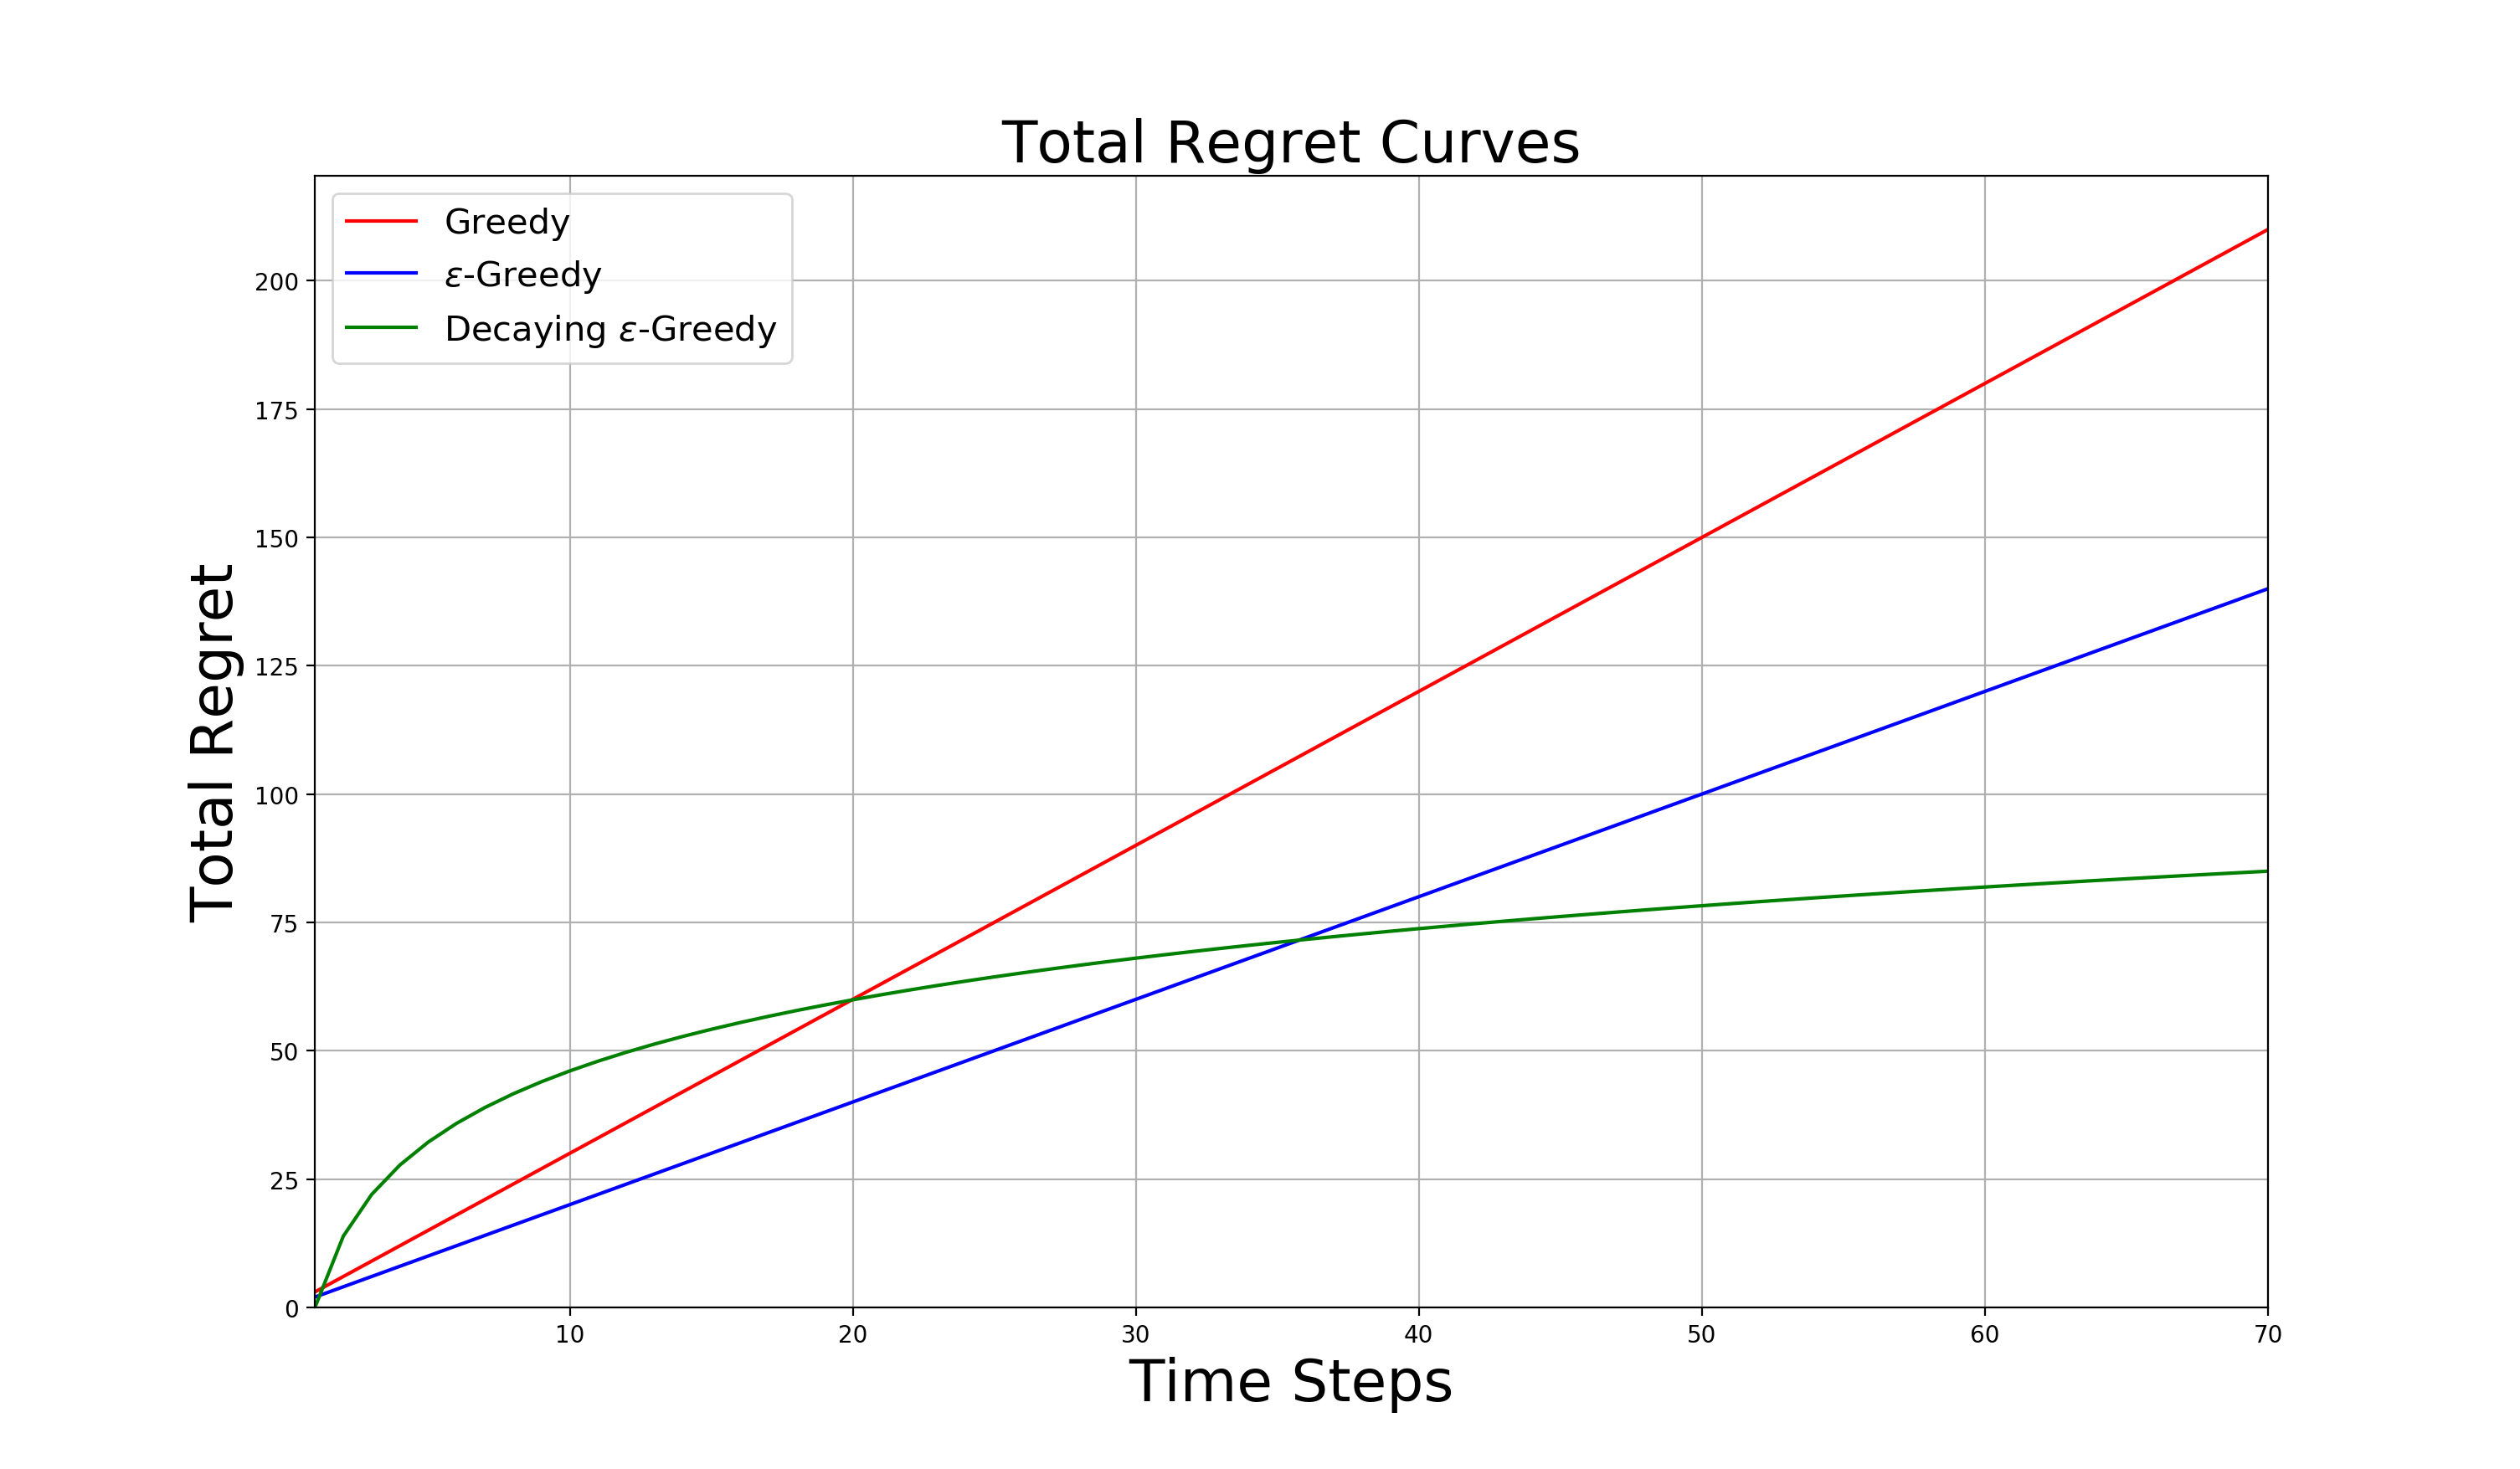
\includegraphics[width=12cm, height=5.5cm]{total_regret_curves.png}
\begin{itemize}
\item If an algorithm {\em never} explores, it will have linear total regret
\item If an algorithm {\em forever} explores, it will have linear total regret
\item Is it possible to achieve sublinear total regret?
\end{itemize}
\end{frame}

\begin{frame}
\frametitle{Greedy Algorithm}
\pause
\begin{itemize}[<+->]
\item We consider algorithms that estimate $\hat{Q}_t(a) \approx Q(a)$
\item Estimate the value of each action by rewards-averaging
$$\hat{Q}_t(a) = \frac 1 {N_t(a)} \sum_{s=1}^t r_s \cdot \mathbbm{1}_{a_s=a}$$
\item The {\em Greedy} algorithm selects the action with highest estimated value
$$a_t = \argmax_{a\in \mathcal{A}} \hat{Q}_{t-1}(a)$$
\item Greedy algorithm can lock onto a suboptimal action forever
\item Hence, Greedy algorithm has linear total regret
\end{itemize}
\end{frame}


\begin{frame}
\frametitle{$\epsilon$-Greedy Algorithm}
\pause
\begin{itemize}[<+->]
\item The $\epsilon$-Greedy algorithm continues to explore forever
\item At each time-step $t$:
\begin{itemize}
\item With probability $1-\epsilon$, select $a_t=\argmax_{a\in\mathcal{A}} \hat{Q}_{t-1}(a)$
\item With probability $\epsilon$, select a random action (uniformly) from $\mathcal{A}$
\end{itemize}
\item Constant $\epsilon$ ensures a minimum regret proportional to mean gap
$$ l_t \geq \frac {\epsilon} {|\mathcal{A}|} \sum_{a\in\mathcal{A}} \Delta_a$$
\item Hence, $\epsilon$-Greedy algorithm has linear total regret
\end{itemize}
\end{frame}


\begin{frame}
\frametitle{Optimistic Initialization}
\pause
\begin{itemize}[<+->]
\item Simple and practical idea: Initialize $\hat{Q}_0(a)$ to a high value for all $a\in \mathcal{A}$
\item Update action value by incremental-averaging
\item Starting with $N_0(a) \geq 0$ for all $a\in \mathcal{A}$,
$$N_t(a) = N_{t-1}(a) + \mathbbm{1}_{a = a_t} \mbox{ for all } a$$
$$\hat{Q}_t(a_t) = \hat{Q}_{t-1}(a_t) + \frac 1 {N_t(a_t)} (r_t - \hat{Q}_{t-1}(a_t))$$
$$\hat{Q}_t(a) = \hat{Q}_{t-1}(a) \mbox{ for all } a \neq a_t$$
\item Encourages systematic exploration early on
\item One can also start with a high value for $N_0(a)$ for all $a \in \mathcal{A}$
\item But can still lock onto suboptimal action
\item Hence, Greedy $+$ optimistic initialization has linear total regret
\item $\epsilon$-Greedy $+$ optimistic initialization also has linear total regret
\end{itemize}
\end{frame}

\begin{frame}
\frametitle{Decaying $\epsilon_t$-Greedy Algorithm}
\pause
\begin{itemize}[<+->]
\item Pick a decay schedule for $\epsilon_1, \epsilon_2, \ldots$
\item Consider the following schedule
$$c > 0$$
$$d = \min_{a|\Delta_a > 0} \Delta_a$$
$$\epsilon_t = \min(1, \frac {c|\mathcal{A}|} {d^2t}\}$$
\item Decaying $\epsilon_t$-Greedy algorithm has {\em logarithmic} total regret
\item Unfortunately, above schedule requires advance knowledge of gaps
\item Practically, implementing {\em some} decay schedule helps considerably
\item \href{https://github.com/TikhonJelvis/RL-book/blob/master/rl/chapter14/epsilon_greedy.py}{\underline{\textcolor{blue}{Educational Code}}} for decaying $\epsilon$-greedy with optimistic initialization
\end{itemize}
\end{frame}



\begin{frame}
\frametitle{Lower Bound}
\pause
\begin{itemize}[<+->]
\item Goal: Find an algorithm with sublinear total regret for any multi-armed bandit (without any prior knowledge of $\mathcal{R}$)
\item The performance of any algorithm is determined by the similarity between the optimal arm and other arms
\item Hard problems have similar-looking arms with different means
\item Formally described by KL-Divergence $KL(\mathcal{R}^a||\mathcal{R}^{a^*})$ and gaps $\Delta_a$
\begin{theorem}[Lai and Robbins]
Asymptotic Total Regret is at least logarithmic in number of steps
$$\lim_{T\rightarrow \infty} L_T \geq \log T \sum_{a|\Delta_a > 0} \frac 1 {\Delta_a}  \geq \log T  \sum_{a|\Delta_a > 0} \frac {\Delta_a} {KL(\mathcal{R}^a||\mathcal{R}^{a^*})}$$
\end{theorem}
\end{itemize}
\end{frame}

\begin{frame}
\frametitle{Optimism in the Face of Uncertainty}
\pause
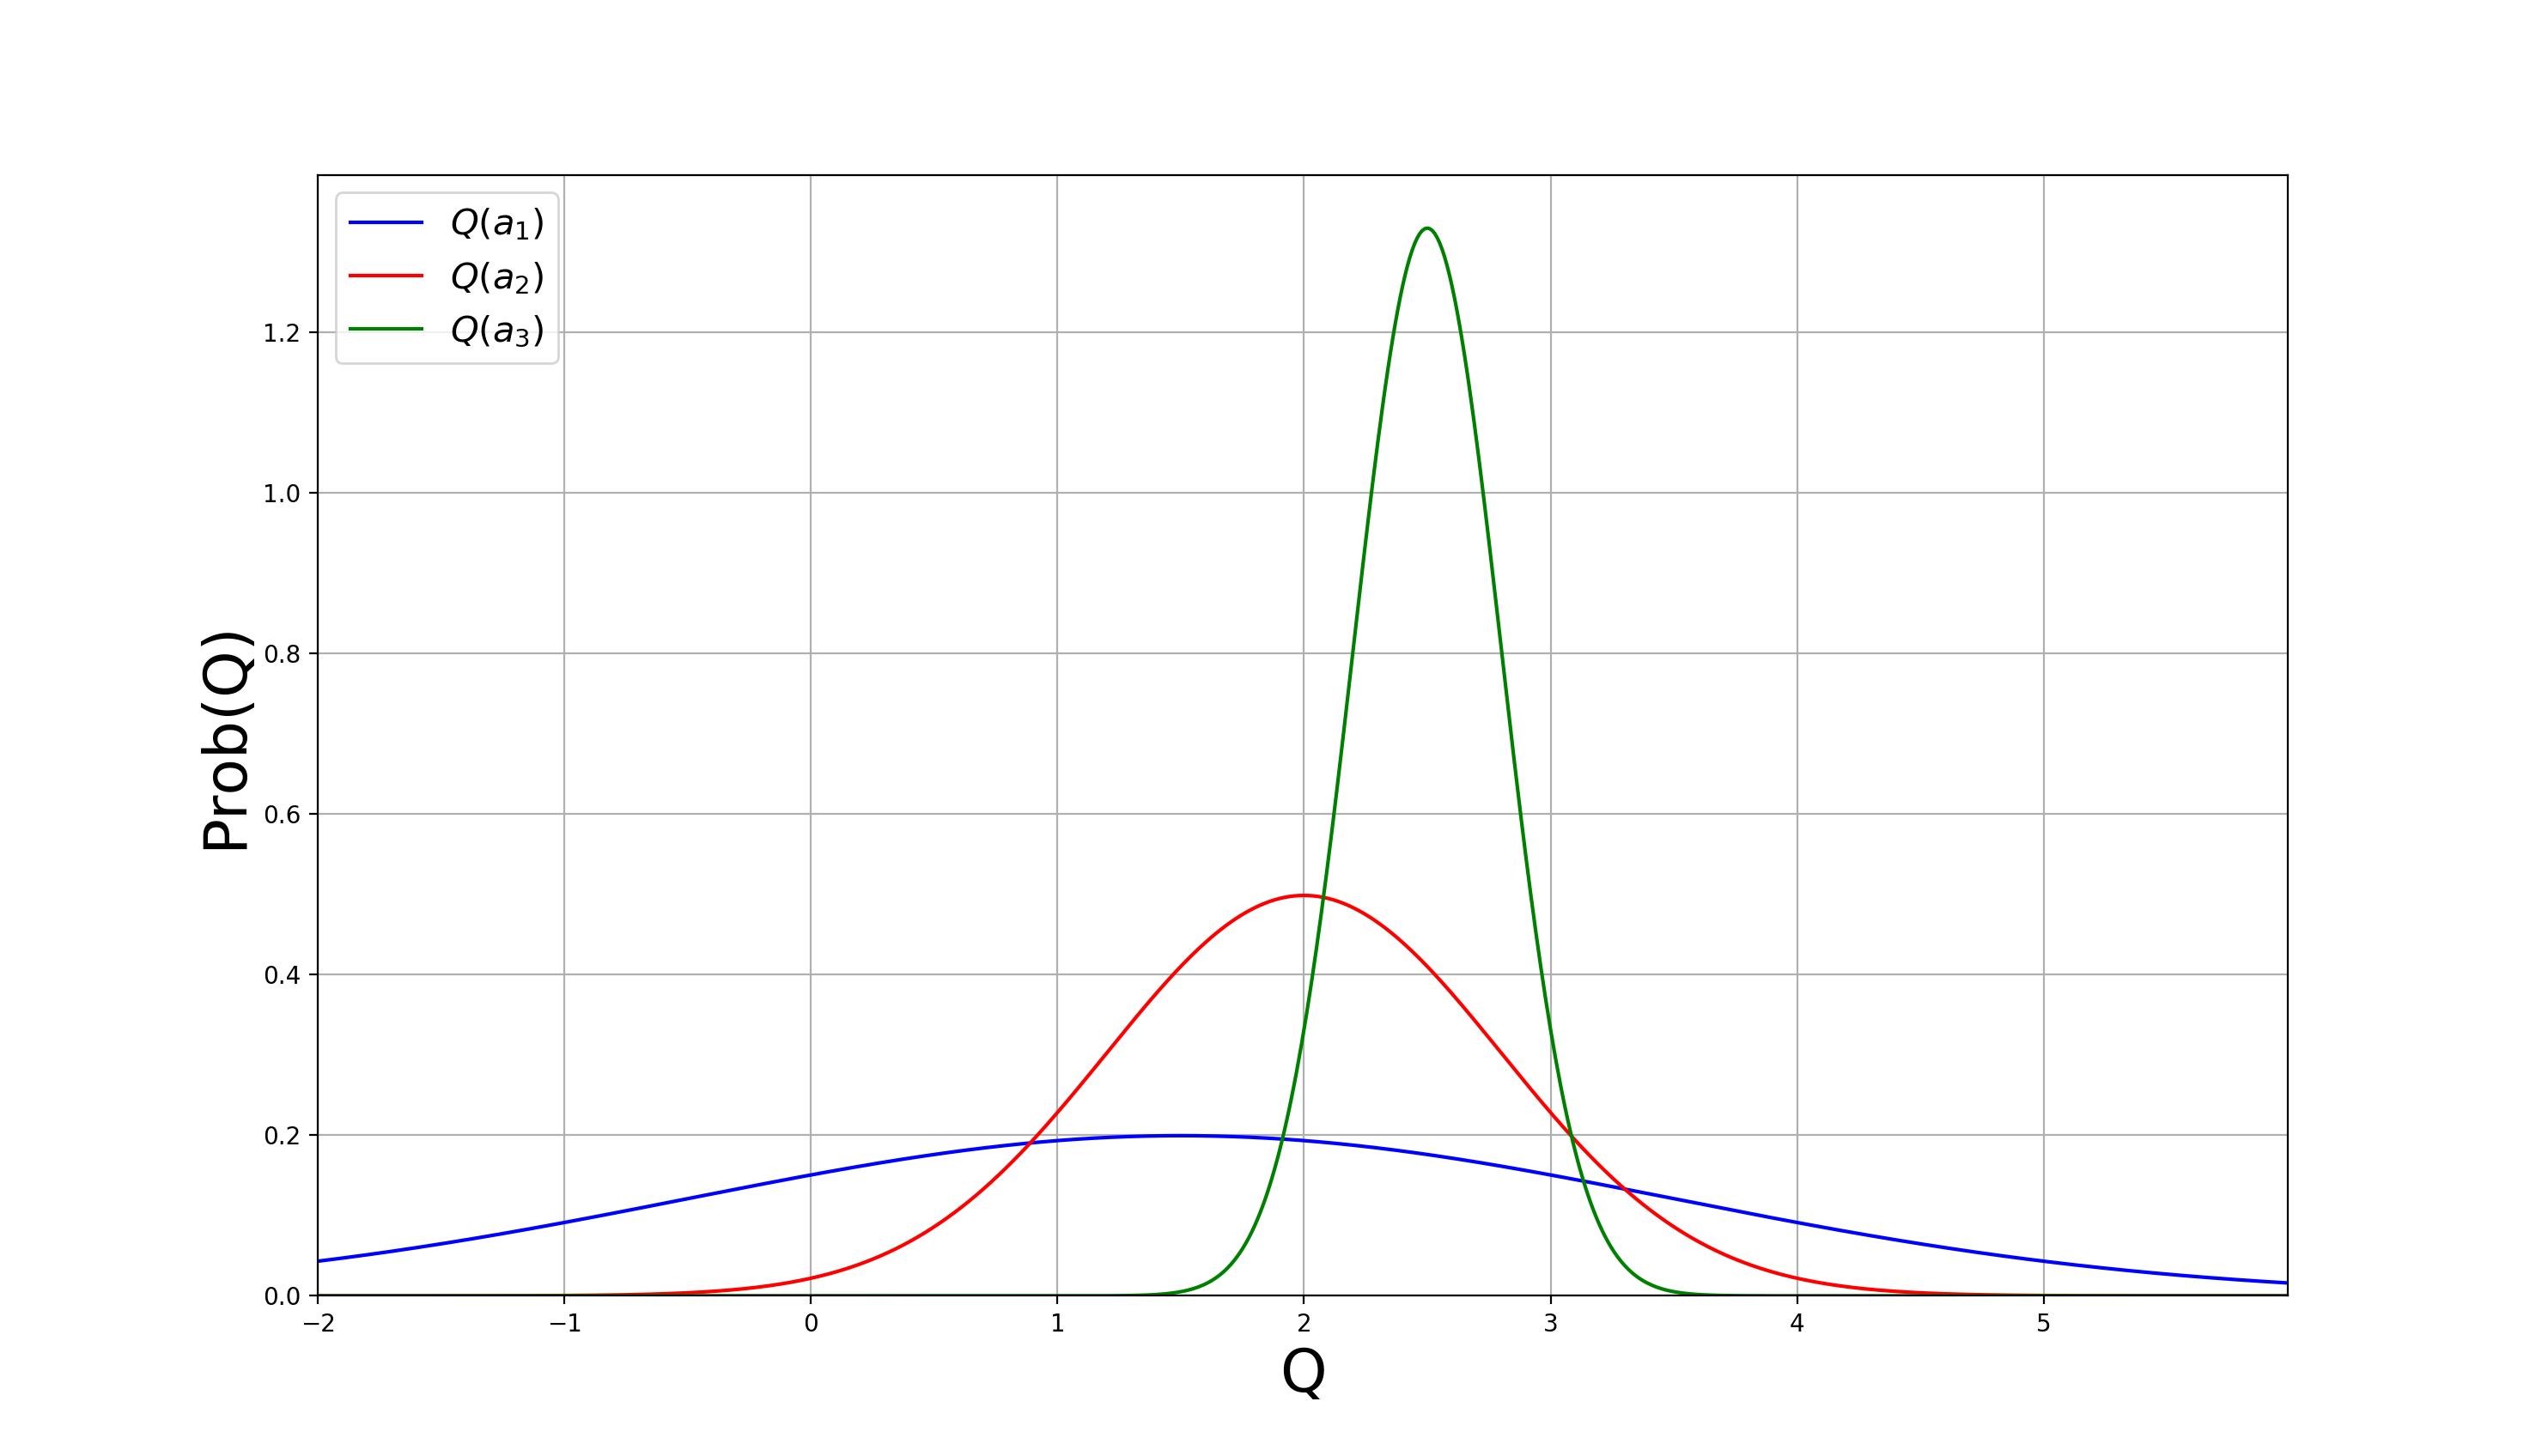
\includegraphics[width=12cm, height=5cm]{q_pdfs1.png}
\begin{itemize}[<+->]
\item Which action should we pick?
\item The more uncertain we are about an action-value, the more important it is to explore that action
\item It could turn out to be the best action
\end{itemize}
\end{frame}

\begin{frame}
\frametitle{Optimism in the Face of Uncertainty (continued)}
\pause
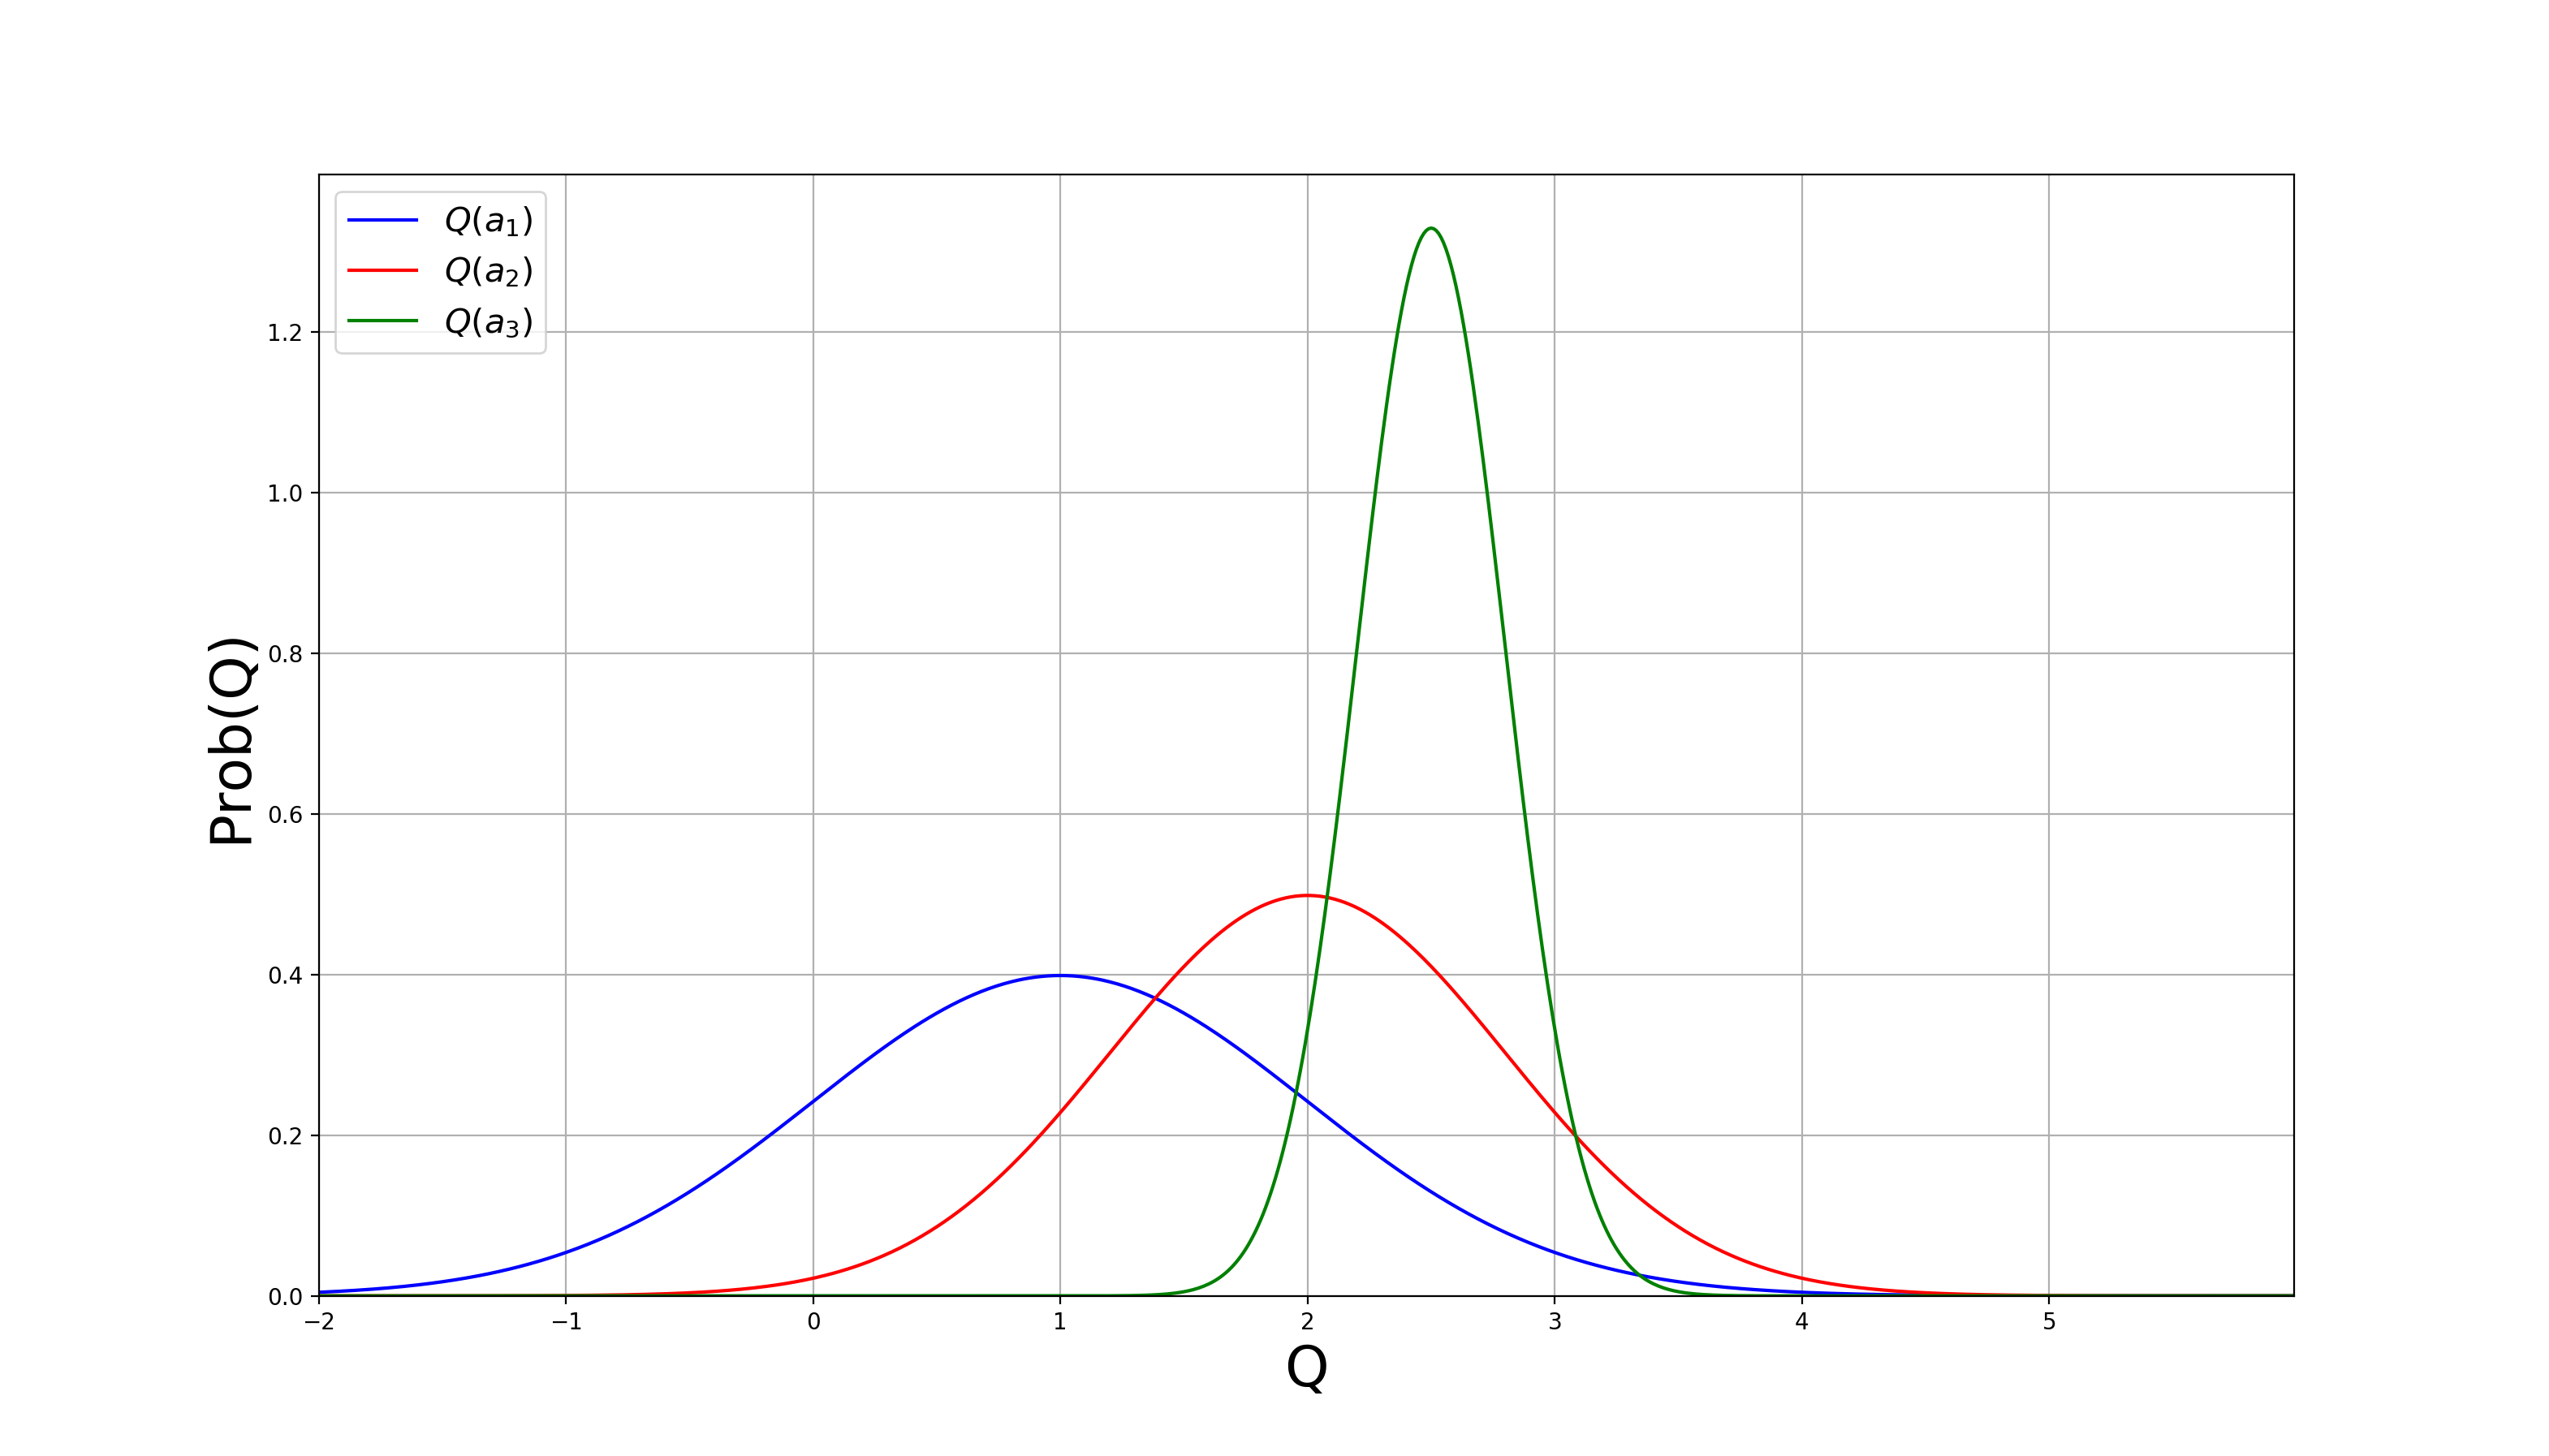
\includegraphics[width=12cm, height=5cm]{q_pdfs2.png}
\begin{itemize}[<+->]
\item After picking {\em blue} action, we are less uncertain about the value
\item And more likely to pick another action
 \item Until we home in on the best action
\end{itemize}
\end{frame}



\begin{frame}
\frametitle{Upper Confidence Bounds}
\pause
\begin{itemize}[<+->]
\item Estimate an upper confidence $\hat{U}_t(a)$ for each action value
\item Such that $Q(a) \leq \hat{Q}_t(a) + \hat{U}_t(a)$ with high probability
\item This depends on the number of times $N_t(a)$ that $a$ has been selected
\begin{itemize}
\item Small $N_t(a) \Rightarrow$ Large $\hat{U}_t(a)$ (estimated value is uncertain)
\item Large $N_t(a) \Rightarrow$ Small $\hat{U}_t(a)$ (estimated value is accurate)
\end{itemize}
\item Select action maximizing Upper Confidence  Bound (UCB)
$$a_{t+1} = \argmax_{a\in\mathcal{A}} \{ \hat{Q}_t(a) + \hat{U}_t(a) \}$$
\end{itemize}
\end{frame}

\begin{frame}
\frametitle{Hoeffding's Inequality}
\pause
\begin{theorem}[Hoeffding's Inequality]
Let $X_1, \ldots, X_n$ be i.i.d. random variables in $[0,1]$, and let $$\bar{X}_n = \frac 1 n \sum_{i=1}^n X_i$$ be the sample mean. Then for any $u \geq 0$,
$$\mathbb{P}[\mathbb{E}[\bar{X}_n] > \bar{X}_n + u] \leq e^{-2nu^2}$$
\end{theorem}
\begin{itemize}[<+->]
\item Apply Hoeffding's Inequality to rewards of $[0,1]$-support bandits
\item Conditioned on selecting action $a$ at time step $t$, setting $n = N_t(a)$ and $u=\hat{U}_t(a)$,
$$\mathbb{P}[Q(a) > \hat{Q}_t(a) + \hat{U}_t(a)] \leq e^{-2N_t(a) \cdot \hat{U}_t(a)^2}$$
\end{itemize}
\end{frame}



\begin{frame}
\frametitle{Calculating Upper Confidence Bounds}
\pause
\begin{itemize}[<+->]
\item Pick a small probability $p$ that $Q(a)$ exceeds UCB $\{\hat{Q}_t(a) + \hat{U}_t(a)\}$
\item Now solve for $\hat{U}_t(a)$
$$e^{-2N_t(a) \cdot \hat{U}_t(a)^2} = p$$
$$\Rightarrow \hat{U}_t(a) = \sqrt{\frac {-\log p} {2 N_t(a)}}$$
\item Reduce $p$ as we observe more rewards, eg: $p = t^{-\alpha}$ (for fixed $\alpha > 0$)
\item This ensures we select optimal action as $t\rightarrow \infty$
$$\hat{U}_t(a) = \sqrt{\frac {\alpha \log t} {2N_t(a)}}$$
\end{itemize}
\end{frame}

\begin{frame}
\frametitle{UCB1}
\pause
Yields UCB1 algorithm for arbitrary-distribution arms bounded in $[0,1]$
$$a_{t+1} = \argmax_{a\in \mathcal{A}} \{ \hat{Q}_t(a) + \sqrt{\frac {\alpha \log t} {2N_t(a)}} \}$$
\begin{theorem}
The UCB1 Algorithm achieves logarithmic total regret
$$L_T \leq \sum_{a|\Delta_a > 0} \frac {4\alpha \cdot \log T} {\Delta_a} + \frac {2\alpha \cdot \Delta_a}{\alpha - 1}$$
\end{theorem}
\href{https://github.com/TikhonJelvis/RL-book/tree/master/rl/chapter14/ucb1.py}{\underline{\textcolor{blue}{Educational Code}}} for UCB1 algorithm
\end{frame}

\begin{frame}
\frametitle{Bayesian Bandits}
\pause
\begin{itemize}
\item So far we have made no assumptions about the rewards distribution $\mathcal{R}$ (except bounds on rewards)
\item {\em Bayesian Bandits} exploit prior knowledge of rewards distribution $\mathbb{P}[\mathcal{R}]$
\item They compute posterior distribution of rewards $\mathbb{P}[\mathcal{R}|h_t]$ where $h_t = a_1,r_1, \ldots, a_t, r_t$ is the history
\item Use posterior to guide exploration
\begin{itemize}
\item Upper Confidence Bounds (Bayesian UCB)
\item Probability Matching (Thompson sampling)
\end{itemize}
\item Better performance if prior knowledge of $\mathcal{R}$ is accurate
\end{itemize}
\end{frame}

\begin{frame}
\frametitle{Bayesian UCB Example: Independent Gaussians}
\pause
\begin{itemize}[<+->]
\item Assume reward distribution is Gaussian, $\mathcal{R}^a(r) =\mathcal{N}(r;\mu_a, \sigma_a^2)$
\item Compute Gaussian posterior over $\mu_a,\sigma_a^2$  (Bayes update details \href{https://people.eecs.berkeley.edu/~jordan/courses/260-spring10/lectures/lecture5.pdf}{\underline{\textcolor{blue}{here}}})
$$\mathbb{P}[\mu_a, \sigma_a^2|h_t] \propto \mathbb{P}[\mu_a, \sigma_a^2] \cdot \prod_{t|a_t=a} \mathcal{N}(r_t;\mu_a, \sigma_a^2)$$
\item Pick action that maximizes Expectation of:  ``$c$ std-errs above mean''
$$a_{t+1} = \argmax_{a\in\mathcal{A}} \mathbb{E}_{\mathbb{P}[\mu_a, \sigma_a|h_t]}[\mu_a + \frac {c \cdot \sigma_a} {\sqrt{N_t(a)}}]$$
\end{itemize}
\end{frame}


\begin{frame}
\frametitle{Probability Matching}
\pause
\begin{itemize}[<+->]
\item {\em Probability Matching} selects action $a$ according to probability that $a$ is the optimal action
$$\pi(a_{t+1}|h_t) = \mathbb{P}_{\mathcal{D}_t\sim \mathbb{P}[\mathcal{R}|h_t]}[\mathbb{E}_{\mathcal{D}_t}[r|a_{t+1}] > \mathbb{E}_{\mathcal{D}_t}[r|a], \forall a \neq a_{t+1}]$$
\item Probability matching is optimistic in the face of uncertainty
\item Because uncertain actions have higher probability of being max
\item Can be difficult to compute analytically from posterior
\end{itemize}
\end{frame}

\begin{frame}
\frametitle{Thompson Sampling}
\pause
\begin{itemize}[<+->]
\item {\em Thompson Sampling} implements probability matching 
$$\pi(a_{t+1}|h_t) = \mathbb{P}_{\mathcal{D}_t\sim \mathbb{P}[\mathcal{R}|h_t]}[\mathbb{E}_{\mathcal{D}_t}[r|a_{t+1}] > \mathbb{E}_{\mathcal{D}_t}[r|a], \forall a \neq a_{t+1}]$$
$$=\mathbb{E}_{\mathcal{D}_t\sim \mathbb{P}[\mathcal{R}|h_t]}[\mathbbm{1}_{a_{t+1}=\argmax_{a\in\mathcal{A}} \mathbb{E}_{\mathcal{D}_t}[r|a]}]$$
\item Use Bayes law to compute posterior distribution $\mathbb{P}[\mathcal{R}|h_t]$
\item {\em Sample} a reward distribution $\mathcal{D}_t$ from posterior $\mathbb{P}[\mathcal{R}|h_t]$
\item Estimate Action-Value function with sample $\mathcal{D}_t$ as $\hat{Q}_t(a) = \mathbb{E}_{\mathcal{D}_t}[r|a]$
\item Select action maximizing value of sample
$$a_{t+1} = \argmax_{a\in\mathcal{A}} \hat{Q}_t(a)$$
\item Thompson Sampling achieves Lai-Robbins lower bound!
\item \href{https://github.com/TikhonJelvis/RL-book/tree/master/rl/chapter14/ts_gaussian.py}{\underline{\textcolor{blue}{Educational Code}}} for Thompson Sampling for Gaussian Distributions
\item \href{https://github.com/TikhonJelvis/RL-book/tree/master/rl/chapter14/ts_bernoulli.py}{\underline{\textcolor{blue}{Educational Code}}} for Thompson Sampling for Bernoulli Distributions
\end{itemize}
\end{frame}

\begin{frame}
\frametitle{Gradient Bandit Algorithms}
\pause
\begin{itemize}[<+->]
\item Gradient Bandit Algorithms are based on Stochastic Gradient Ascent
\item We optimize {\em Score} parameters $s_a$ for $a\in \mathcal{A} = \{a_1, \ldots, a_m\}$
\item Objective function to be maximized is the Expected Reward
$$J(s_{a_1}, \ldots, s_{a_m}) = \sum_{a\in\mathcal{A}} \pi(a) \cdot \mathbb{E}[r|a]$$
\item $\pi(\cdot)$ is probabilities of taking actions (based on a stochastic policy)
\item The stochastic policy governing $\pi(\cdot)$ is a function of the {\em Scores}:
$$\pi(a) = \frac {e^{s_a}} {\sum_{b\in \mathcal{A}} e^{s_b}}$$
\item {\em Scores} represent the relative value of actions based on seen rewards
\item Note: $\pi$ has a Boltzmann distribution (Softmax-function of {\em Scores})
\item We move the {\em Score} parameters $s_a$ (hence, action probabilities $\pi(a)$) 
such that we ascend along the direction of gradient of objective $J(\cdot)$
\end{itemize}
\end{frame}

\begin{frame}
\frametitle{Gradient of Expected Reward}
\pause
\begin{itemize}[<+->]
\item To construct Gradient of $J(\cdot)$, we calculate $\pderiv{J}{s_a}$ for all $a\in \mathcal{A}$
$$\pderiv{J}{s_a} = \pderiv{}{s_a}(\sum_{a'\in\mathcal{A}} \pi(a') \cdot \mathbb{E}[r|a'])
 = \sum_{a'\in\mathcal{A}} \mathbb{E}[r|a'] \cdot \pderiv{\pi(a')} {s_a}$$ 
$$ = \sum_{a'\in\mathcal{A}} \pi(a') \cdot \mathbb{E}[r|a'] \cdot \pderiv{\log \pi(a')} {s_a} 
= \mathbb{E}_{a'\sim \pi, r\sim \mathcal{R}^{a'}}[r \cdot \pderiv{\log \pi(a')} {s_a}]$$
\item We know from standard softmax-function calculus that:
$$\pderiv{\log \pi(a')} {s_a} = \pderiv{}{s_a}(\log\frac {e^{s_{a'}}} {\sum_{b\in \mathcal{A}} e^{s_b}}) = \mathbbm{1}_{a=a'} - \pi(a)$$
\item Therefore $\pderiv{J}{s_a}$ can we re-written as:
$$=\mathbb{E}_{a'\sim \pi, r\sim \mathcal{R}^{a'}}[r \cdot  (\mathbbm{1}_{a=a'} - \pi(a))]$$
\item At each step $t$, we approximate the gradient with $(a_t, r_t)$ sample as:
$$r_t \cdot (\mathbbm{1}_{a=a_t} - \pi_t(a)) \mbox{ for all } a \in \mathcal{A}$$
\end{itemize}
\end{frame}

\begin{frame}
\frametitle{Score updates with Stochastic Gradient Ascent}
\pause
\begin{itemize}[<+->]
\item $\pi_t(a)$ is the probability of $a$ at step $t$ derived from score $s_t(a)$ at step $t$
\item Reduce variance of estimate with baseline $B$ that's independent of $a$:
$$(r_t -B) \cdot (\mathbbm{1}_{a=a_t} - \pi_t(a)) \mbox{ for all } a \in \mathcal{A}$$
\item This doesn't introduce bias in the estimate of gradient of $J(\cdot)$ because
$$\mathbb{E}_{a'\sim \pi}[B \cdot (\mathbbm{1}_{a=a'} - \pi(a))] = \mathbb{E}_{a'\sim \pi}[B \cdot \pderiv{\log \pi(a')} {s_a}]$$
$$= B \cdot \sum_{a'\in\mathcal{A}} \pi(a') \cdot \pderiv{\log \pi(a')} {s_a} = B \cdot \sum_{a'\in\mathcal{A}} \pderiv{\pi(a')} {s_a} = B \cdot \pderiv{}{s_a}(\sum_{a'\in\mathcal{A}} \pi(a')) = 0$$
\item We can use $B = \bar{r_t} =\frac 1 t \sum_{s=1}^t r_s = $ average rewards until step $t$
\item So, the update to scores $s_t(a)$ for all $a\in\mathcal{A}$ is: 
$$s_{t+1}(a) = s_t(a) + \alpha \cdot (r_t - \bar{r_t}) \cdot (\mathbbm{1}_{a=a_t} - \pi_t(a))$$
\item \href{https://github.com/TikhonJelvis/RL-book/tree/master/rl/chapter14/gradient_bandits.py}{\underline{\textcolor{blue}{Educational Code}}} for this Gradient Bandit Algorithm
\end{itemize}
\end{frame}



\begin{frame}
\frametitle{Value of Information}
\pause
\begin{itemize}[<+->]
\item Exploration is useful because it gains information
\item Can we quantify the value of information?
\begin{itemize}
\item How much would a decision-maker be willing to pay to have that information, prior to making a decision?
\item Long-term reward after getting information minus immediate reward 
\end{itemize}
\item Information gain is higher in uncertain situations
\item Therefore it makes sense to explore uncertain situations more
\item If we know value of information, we can trade-off exploration and exploitation {\em optimally}
\end{itemize}
\end{frame}

\begin{frame}
\frametitle{Information State Space}
\pause
\begin{itemize}[<+->]
\item We have viewed bandits as {\em one-step} decision-making problems
\item Can also view as {\em sequential} decision-making problems
\item At each step there is an {\em information state} $\tilde{s}$
\begin{itemize}
\item $\tilde{s}$ is a statistic of the history, i.e., $\tilde{s}_t = f(h_t)$
\item summarizing all information accumulated so far
\end{itemize}
\item Each action $a$ causes a transition to a new information state $\tilde{s}'$ (by adding information), with probability $\tilde{\mathcal{P}}_{\tilde{s},\tilde{s}'}^a$
\item This defines an MDP $\tilde{M}$ in information state space
$$\tilde{M} = (\tilde{\mathcal{S}}, \mathcal{A}, \tilde{\mathcal{P}}, \mathcal{R}, \gamma)$$
\end{itemize}
\end{frame}

\begin{frame}
\frametitle{Example: Bernoulli Bandits}
\pause
\begin{itemize}[<+->]
\item Consider a Bernoulli Bandit, such that $\mathcal{R}^a = \mathcal{B}(\mu_a)$
\item For arm $a$, reward=1 with probability $\mu_a$ (=0 with probability $1-\mu_a$)
\item Assume we have $m$ arms $a_1, a_2, \ldots, a_m$
\item The information state is $\tilde{s} = (\alpha_{a_1}, \beta_{a_1}, \alpha_{a_2}, \beta_{a_2}\ldots, \alpha_{a_m}, \beta_{a_m})$
\item $\alpha_a$ records the pulls of arms $a$  for which reward was 1
\item $\beta_a$ records the pulls of arm $a$ for which reward was 0
\item In the long-run, $\frac {\alpha_a} {\alpha_a + \beta_a} \rightarrow \mu_a$
\end{itemize}
\end{frame}

\begin{frame}
\frametitle{Solving Information State Space Bandits}
\pause
\begin{itemize}[<+->]
\item We now have an infinite MDP over information states
\item This MDP can be solved by Reinforcement Learning
\item Model-free Reinforcement learning, eg: Q-Learning (Duff, 1994)
\item Or Bayesian Model-based Reinforcement Learning
\begin{itemize}
\item eg: Gittins indices (Gittins, 1979)
\item This approach is known as Bayes-adaptive RL
\item Finds Bayes-optimal exploration/exploitation trade-off with respect of prior distribution
\end{itemize}
\end{itemize}
\end{frame}

\begin{frame}
\frametitle{Bayes-Adaptive Bernoulli Bandits}
\pause
\begin{itemize}[<+->]
\item Start with $Beta(\alpha_a, \beta_a)$ prior over reward function $\mathcal{R}^a$
\item Each time $a$ is selected, update posterior for $\mathcal{R}^a$ as:
\begin{itemize}
\item $Beta(\alpha_a+1, \beta_a)$ if $r=1$
\item $Beta(\alpha_a, \beta_a+1)$ if $r=0$
\end{itemize}
\item This defines transition function $\tilde{\mathcal{P}}$ for the Bayes-adaptive MDP
\item $(\alpha_a, \beta_a)$ in information state provides reward model $Beta(\alpha_a, \beta_a)$
\item Each state transition corresponds to a Bayesian model update
\end{itemize}
\end{frame}

\begin{frame}
\frametitle{Gittins Indices for Bernoulli Bandits}
\pause
\begin{itemize}[<+->]
\item Bayes-adaptive MDP can be solved by Dynamic Programming
\item The solution is known as the Gittins Index
\item Exact solution to Bayes-adaptive MDP is typically intractable
\item Guez et al. 2020 applied Simulation-based search
\begin{itemize}
\item Forward search in information state space
\item Using simulations from current information state
\end{itemize}
\end{itemize}
\end{frame}

\begin{frame}
\frametitle{Summary of approaches to Bandit Algorithms}
\pause
\begin{itemize}[<+->]
\item Naive Exploration (eg: $\epsilon$-Greedy)
\item Optimistic Initialization
\item Optimism in the face of uncertainty (eg: UCB, Bayesian UCB)
\item Probability Matching (eg: Thompson Sampling)
\item Gradient Bandit Algorithms
\item Information State Space MDP, incorporating value of information
\end{itemize}
\end{frame}


\begin{frame}
\frametitle{Contextual Bandits}
\pause
\begin{itemize}[<+->]
\item A Contextual Bandit is a 3-tuple $(\mathcal{A}, \mathcal{S},  \mathcal{R})$
\item $\mathcal{A}$ is a known set of $m$ actions (``arms'')
\item $\mathcal{S} = \mathbb{P}[s]$ is an {\bf unknown} distribution over states (``contexts'')
\item $\mathcal{R}^a_s(r) = \mathbb{P}[r|s,a]$ is an {\bf unknown} probability distribution over rewards
\item At each step $t$, the following sequence of events occur:
\begin{itemize}
\item The environment generates a states $s_t \sim \mathcal{S}$
\item Then the AI Agent (algorithm) selects an actions $a_t \in \mathcal{A}$
\item Then the environment generates a reward $r_t \in \mathcal{R}^{a_t}_{s_t}$
\end{itemize}
\item The AI agent's goal is to maximize the Cumulative Reward:
$$\sum_{t=1}^T r_t$$
\item Extend Bandit Algorithms to Action-Value $Q(s,a)$ (instead of $Q(a)$)
\end{itemize}
\end{frame}



\end{document}
